% conceitos basicos
Neste capítulo faremos uma apresentação dos conceitos básicos
necessários para o entendimento e desenvolvimento deste trabalho. Na
Seção \ref{sec:defin} mostraremos as definições usadas no decorrer
deste trabalho. As seções \ref{sec:rev}, \ref{sec:trans}
e \ref{sec:rev_trans} descrevem, respectivamente, os problemas de
ordenação por reversões, ordenação por transposições e ordenação por
reversões e transposições. A Seção \ref{sec:def_cp} explica o conceito
de \pr{}.

\section{Definições}
\label{sec:defin}
Para todos os problemas usamos as seguintes definições.

\textit{Permutação.} 
Para fins computacionais, um genoma é representado por uma $n$-tupla
de genes, e quando não há genes repetidos essa $n$-tupla é chamada de
permutação. Uma permutação é representada como $\pi =
(\pi_{1}~\pi_{2}~\ldots~\pi_{n})$, para $\pi_{i} \in \mathbb{N}$, $0
< \pi_{i} \leq n$ e $i \neq j \leftrightarrow \pi_{i} \neq \pi_{j}$. A
permutação identidade é representada como $\iota =
(1~2~3~\ldots~n)$. Para a demonstração dos eventos, usaremos como
base a permutação $\pi = (4~7~3~6~2~5~1)$.

\textit{Eventos de rearranjo.}
Os eventos de rearranjo tratados neste trabalho são os eventos de
transposição e reversão quando ocorrem isoladamente e quando ocorrem
de forma conjunta. Os eventos são representados por $\rho$ e são
aplicados a $\pi$ de uma maneira específica.

\section{Ordenação por Reversões}
\label{sec:rev}
Um evento de reversão ocorre quando um bloco do genoma é
invertido. Uma reversão $\rho(i, j)$, para $1 \leq i < j \leq n$,
aplicada ao genoma $\pi = (\pi_{1}~\pi_{2}~\ldots~\pi_{n})$ gera a
permutação $\pi\rho =
(\pi_{1}~\ldots~\pi_{i-1}~\pi_{j}~\pi_{j-1}~\ldots~\pi_{i+1}$
$\pi_{i}~ \pi_{j+1}~\ldots~\pi_{n})$, caso a orientação de $\pi$ não
seja conhecida (Figura~\ref{fig:rev_nao_orientada}), e $\pi\rho =
(\pi_{1}~\ldots~\pi_{i-1}~-\pi_{j}~-\pi_{j-1}~\ldots~-\pi_{i+1}$
$-\pi_{i}~ \pi_{j+1}~\ldots~\pi_{n})$, caso a orientação de $\pi$ seja
conhecida (Figura~\ref{fig:rev_orientada}).

\begin{figure}
  \centering
  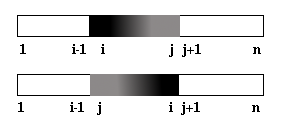
\includegraphics{images/rev_nao_orientada.png} 
  \caption{Reversão em uma permutação não orientada.}
  \label{fig:rev_nao_orientada}
\end{figure}

\begin{figure}
  \centering
  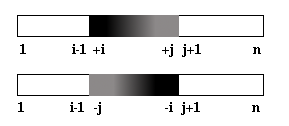
\includegraphics{images/rev_orientada.png}
  \caption{Reversão em uma permutação orientada.}
  \label{fig:rev_orientada}
\end{figure}

A distância de reversão $d_{r}(\pi,\sigma)$ entre duas permutações
$\pi$ e $\sigma$ é o número mínimo $r$ de reversões $\rho_{1}$,
$\rho_{2}$,~$\ldots$~, $\rho_{r}$ tal que
$\pi \rho_{1} \rho_{2}~\ldots~\rho_{r} = \sigma$. Note que a distância
de reversão entre $\pi$ e $\sigma$ é igual à distância de reversão
entre $\sigma^{-1} \pi$ e $\iota$. Então, sem perda de generalidade,
podemos dizer que o problema da distância de reversão é equivalente ao
problema de ordenação por reversões, que é a distância de reversão
entre a permutação $\pi$ e a permutação identidade $\iota$, denotado
por $d_{r}(\pi)$.

Em um estudo inicial sobre este problema, Bafna e
Pevzner~\cite{BafnaPevzner*1996} apresentaram um algoritmo de
aproximação com razão $1.5$ quando a orientação de genes é conhecida e
$1.75$, caso contrário.

Conhecer a orientação dos genes em um genoma é um fator importante no
problema de reversão, pois existem algoritmos polinomiais para o caso
em que a orientação é conhecida. No caso em que não se conhece a
orientação dos genes, o problema de encontrar a distância de reversão
pertence à classe dos problemas NP-Difíceis~\cite{Caprara*1997}.

O primeiro algoritmo polinomial para o problema de reversão com
orientação conhecida foi criado por Hannenhalli e
Pevzner~\cite{HannenhalliPevzner*1995} que fez uso de várias operações
aplicadas a uma estrutura intermediária conhecida como grafo
de \bkp{}. A estratégia usada por Hannenhalli e Pevzner foi
simplificada no trabalho de Bergeron~\cite{Bergeron*2005}. Atualmente
já existe um algoritmo com complexidade
sub quadrática~\cite{TannierSagot*2004} e, quando apenas a distância é
necessária, um algoritmo linear pode ser
usado~\cite{BaderMoretYan*2001}.

Um resultado importante obtido por Meidanis, Walter e
Dias~\cite{MeidanisWalterDias*2000}, mostrou que toda teoria sobre
reversões desenvolvida para genomas lineares pode ser adaptada
facilmente para genomas circulares, que são comuns em seres inferiores
como vírus e bactérias.

Quando a orientação dos genes não é conhecida, existem algoritmos de
aproximação que seguiram a ideia do trabalho de Bafna e Pevzner citado
anteriormente como, por exemplo, o algoritmo implementado por Berman,
Hannenhalli e Karpinski~\cite{BermanHannenhalliKarpinski*2002} com
razão de aproximação de $1.375$.

\subsection{Ferramentas para o Problema de Ordenação por Reversões}
\label{subsec:toolrev}
O conceito de grafo de \bkp{} foi introduzido no trabalho de Bafna e
Pevzner~\cite{BafnaPevzner*1996}. Inicialmente a permutação $\pi$ é
estendida adicionando o elemento $\pi_{0} = 0$ e $\pi_{n+1} =
n+1$. Dois elementos consecutivos $\pi_{i}$ e $\pi_{i+1}$, $0 \le
i \le n$, são \textit{adjacentes} quando $|\pi_{i} - \pi_{i+1}| = 1$,
e são \estr{breakpoints} caso contrário. Define-se um grafo de arestas
coloridas $G(\pi)$ com $n + 2$ vértices \{0, 1,~$\ldots$~, $n$, $n +
1$\}. Unimos os vértices $i$ e $j$ com uma aresta preta se $(i, j)$
for um \estr{breakpoint}. Unimos os vértices $i$ e $j$ com uma aresta
cinza se $|i - j| = 1$ e $i$, $j$ não são consecutivos em
$\pi$. Denotamos por $b_r(\pi)$ o número de \bkp{} existentes em
$\pi$. A Figura~\ref{fig:rev_grafo_bkp} mostra o grafo de \bkp{} da
permutação $\pi = (4~7~3~6~2~5~1)$.

\begin{figure}[h]
  \centering 
  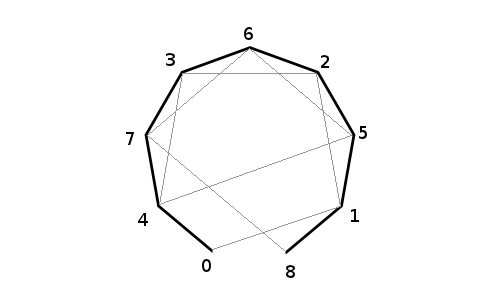
\includegraphics[scale=0.6]{images/rev_grafo_bkp.png} 
  \caption{Grafo de \bkp{} da permutação $\pi = (4~7~3~6~2~5~1)$.}
  \label{fig:rev_grafo_bkp}
\end{figure}

Usando o conceito de \bkp{}, temos que uma reversão atua em dois
pontos em uma permutação e, portanto, pode reduzir o número de \bkp{}
em pelo menos um e no máximo dois~\cite{BafnaPevzner*1996}, levando ao
Teorema~\ref{teo:rev_bkp_bound}. 

\begin{teo}
\label{teo:rev_bkp_bound}
Para qualquer permutação $\pi$, 
\[\frac{1}{2} b_r(\pi) \leq d_r(\pi) \leq
  b_r(\pi).
\]
\end{teo}

Um ciclo em $G(\pi)$ é chamado de \textit{alternado} se as cores de
duas arestas consecutivas são diferentes ao longo do ciclo. Assim
dizemos que todos os ciclos pertencentes ao grafo serão ciclos
alternados. O \textit{comprimento} de um ciclo é a sua quantidade de
arestas pretas. Um $k$-ciclo é um ciclo que contém $k$ arestas
pretas. Um \textit{ciclo longo} é um ciclo de comprimento maior que
dois.

Observe que $G(\pi)$ pode ser decomposto em ciclos de arestas
disjuntas, pois cada vértice tem o mesmo número de arestas incidentes
cinzas e pretas. Logo existem diversas maneiras de realizar a
decomposição de ciclos em $G(\pi)$. A
Figura~\ref{fig:rev_grafo_bkp_dec2cic} mostra um exemplo de
decomposição em ciclos para o grafo de \bkp{} da permutação $\pi =
(4~7~3~6~2~5~1)$.

\begin{figure}[h]
  \centering 
  \begin{tabular}{ccc} 
  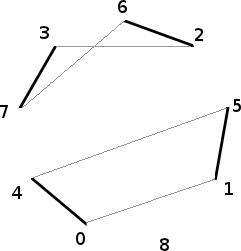
\includegraphics[scale=0.6]{images/rev_grafo_bkp_dec2cic-1.png}
  & ~~~~
  & 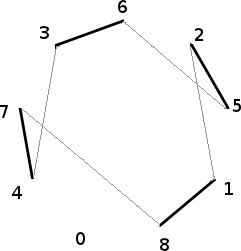
\includegraphics[scale=0.6]{images/rev_grafo_bkp_dec2cic-2.png} 
  \end{tabular} 
  \caption{Exemplo de decomposição em ciclos de arestas disjuntas para
  o grafo de \bkp{} da permutação $\pi = (4~7~3~6~2~5~1)$.}
  \label{fig:rev_grafo_bkp_dec2cic}
\end{figure}

Uma reversão atua em duas arestas pretas de $G(\pi)$, se estas arestas
representam os \bkp{} que são separados pela operação de
reversão~\cite{Christie*1998}. O Teorema~\ref{teo:rev_cic_bound},
demonstrado no trabalho de Christie~\cite{Christie*1998}, fornece os
limitantes para a distância de reversão usando a quantidade de
$2$-ciclos na máxima decomposição em ciclos de $G(\pi)$.

\begin{teo}
\label{teo:rev_cic_bound}
Se $c_{2}(\pi)$ é o número mínimo de $2$-ciclos em qualquer máxima
decomposição em ciclos de $G(\pi)$ então: 
\[
\frac{2}{3} b_r(\pi)
- \frac{1}{3} c_{2}(\pi) \leq d_r(\pi) \leq b_r(\pi) - \frac{1}{2}
c_{2}(\pi).
\]
\end{teo}

\section{Ordenação por Transposições}
\label{sec:trans}
% transposicoes
Um evento de transposição ocorre quando dois blocos adjacentes no
genoma trocam de posição. Uma transposição $\rho(i, j, k)$, para
$1 \leq i < j < k \leq n + 1$, aplicada ao genoma $\pi =
(\pi_{1}~\pi_{2}~\ldots~\pi_{n})$ gera a permutação $\pi\rho =
(\pi_{1}~\ldots~\pi_{i-1}~\pi_{j}~\ldots~\pi_{k-1}~\pi_{i}~\ldots$
$\pi_{j-1}~\pi_{k}~\ldots~\pi_{n})$ (Figura~\ref{fig:transposition}).

\begin{figure}[h]
  \centering
  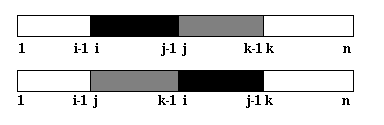
\includegraphics{images/transposition.png} 
  \caption{Transposição aplicada em uma permutação.}
  \label{fig:transposition}
\end{figure}

A distância de transposição $d_{t}(\pi, \sigma)$ entre duas
permutações $\pi$ e $\sigma$ é o número mínimo $t$ de transposições
$\rho_{1}, \rho_{2}, \ldots, \rho_{t}$ tal que
$\pi \rho_{1} \rho_{2} \ldots \rho_{t} = \sigma$. Note que a distância
de transposição entre $\pi$ e $\sigma$ é igual à distância de transposição
entre $\sigma^{-1} \pi$ e $\iota$. Então, sem perda de generalidade,
podemos dizer que o problema da distância de transposição é
equivalente ao problema de ordenação por transposições, que é a
distância de transposição entre a permutação $\pi$ e a permutação
identidade $\iota$, denotado por $d_{t}(\pi)$.

Este problema foi estudado por Bafna e
Pevzner~\cite{BafnaPevzner*1998}, onde apresentaram um algoritmo capaz
de fornecer uma resposta aproximada na razão de $1.5$, além de derivar
um importante limitante inferior para o problema. Introduziram também
o conceito de \bkp{} em eventos de transposições, elementos adjacentes
em um genoma, mas não no outro, e o conceito de grafo de ciclos, ambos
ferramentas importantes utilizadas para encontrar limitantes para o
problema. Foram apresentadas várias questões em aberto, como verificar
a complexidade do problema da distância de transposição e o diâmetro,
que é a maior distância possível entre duas permutações de tamanho
$n$. O problema do diâmetro foi estudado por Meidanis, Walter e
Dias~\cite{MeidanisWalterDias*1997}.

A complexidade deste problema ficou em aberto por um longo tempo. O
trabalho de Bulteau, Fertin e Rusu~\cite{BulteauFertinRusu*2010}
apresentou a prova de que o problema de ordenação por transposição
pertence a classe dos problemas NP-Difíceis. Elias e
Hartman~\cite{EliasHartman*2006} apresentaram um algoritmo de
aproximação na razão de $1.375$. O trabalho de
Labarre~\cite{Labarre*2006} apresentou novos limitantes, além de
definir classes de permutações em que a distância de transposição pode
ser calculada em tempo e espaço lineares.

\subsection{Ferramentas para o Problema de Ordenação por Transposições}
\label{subsec:tooltra}
No problema de ordenação por transposições, um \bkp{} é um par
$(\pi_{i}, \pi_{i+1})$ tal que $\pi_{i+1} \neq \pi_{i} + 1$. Denota-se
por $b_{t}(\pi)$ como sendo o número de \bkp{} na permutação
$\pi$. Sabemos que uma transposição atua em três pontos de uma
permutação, logo, pode reduzir o número de \bkp{} em pelo menos um e
no máximo três~\cite{BafnaPevzner*1998}, levando ao
Teorema~\ref{teo:trans_br_bound}.

\begin{teo}
  \label{teo:trans_br_bound}
  Para qualquer permutação $\pi$, 
  \[
  \frac{1}{3}b_t(\pi) \leq d_t(\pi) \leq b_t(\pi).
  \]
\end{teo}

O conceito de grafo de ciclos foi introduzido por Bafna e
Pevzner~\cite{BafnaPevzner*1998} e foi usado para obter limitantes
melhores para o problema. Um grafo direcionado com arestas coloridas,
denotado por $G(\pi)$, é chamado de grafo de ciclos da permutação
$\pi$ se possui um conjunto de vértices $\{0,~1,~\ldots,~n+1\}$ e seu
conjunto de arestas é definido como para todo $1 \leq i \leq n+1$,
arestas cinzas são direcionadas de $i-1$ para $i$ e arestas pretas de
$\pi_{i}$ para $\pi_{i-1}$. A Figura~\ref{fig:trans_cycle_graph}
mostra o grafo de ciclos para a permutação $\pi = (4~7~3~6~2~5~1)$.

\begin{figure}[h]
  \centering 
  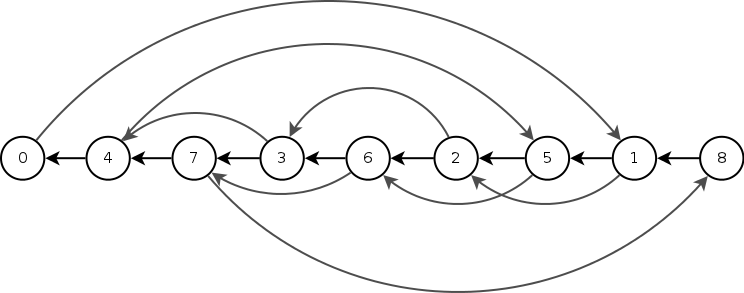
\includegraphics[scale=0.6]{images/trans_cycle_graph.png} 
  \caption{Grafo de ciclos para a permutação $\pi = (4~7~3~6~2~5~1)$.}
  \label{fig:trans_cycle_graph}
\end{figure}

Similar ao problema de ordenação por reversões, um ciclo de $G(\pi)$ é
chamado de \textit{alternado} se ele for um ciclo direcionado com
arestas de cores alternadas. Para todo vértice de $G(\pi)$ toda aresta
chegando é unicamente pareada com uma aresta saindo de cor
diferente. Isto implica que existe uma decomposição única de ciclos
alternados do conjunto de arestas de $G(\pi)$. A seguir o termo ciclo
é usado no lugar de ciclos alternados e usamos o termo $k$-ciclo para
definir um ciclo alternado de tamanho $2k$, $k$-ciclo é longo se $k >
2$, e curto caso contrário. A Figura~\ref{fig:tra_grafo_bkp_dec}
mostra um exemplo de decomposição em ciclos para o grafo de ciclos da
permutação $\pi = (4~7~3~6~2~5~1)$.


\begin{figure}[h]
  \centering 
  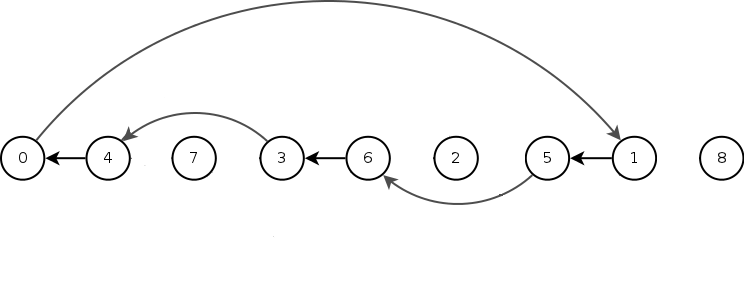
\includegraphics[scale=0.6]{images/trans_cycle_graph_dec-1.png}
  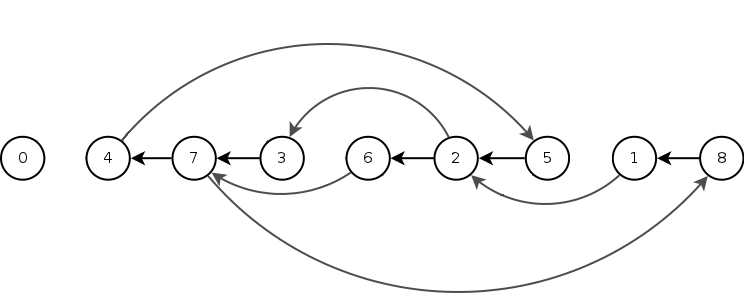
\includegraphics[scale=0.6]{images/trans_cycle_graph_dec-2.png} 
  \caption{Exemplo de decomposição em ciclos de arestas disjuntas para
  o grafo de ciclos da permutação $\pi = (4~7~3~6~2~5~1)$.}
  \label{fig:tra_grafo_bkp_dec}
\end{figure}

Para melhorar o limitante, Bafna e Pevzner~\cite{BafnaPevzner*1998}
estudou separadamente os ciclos pares e ímpares. Um ciclo é impar se
possui um número ímpar de arestas pretas e par caso contrário. Seja
$c_{\text{ímpar}}(\pi)$ o número de ciclos ímpares de $G(\pi)$, para
uma permutação $\pi$, e $\Delta c_{\text{ímpar}} (\rho) =
c_{\text{ímpar}} (\pi \rho) - c_{\text{ímpar}} (\pi)$ a mudança no
número de ciclos ímpares devido a transposição $\rho$, temos que
$\Delta c_{\text{ímpar}} \in \{2, 0, -2\}$, gerando o resultado do
Teorema~\ref{teo:trans_cg_bound}.

\begin{teo} 
  \label{teo:trans_cg_bound} 
  Para qualquer permutação $\pi$, 
  \[ 
  \frac{1}{2}(n + 1 - c_{\text{ímpar}}(\pi)) \leq d_t(\pi) \leq \frac{3}{4} (n
  + 1 - c_{\text{ímpar}}(\pi)).
  \]
\end{teo}

\section{Ordenação por Reversões e Transposições}
\label{sec:rev_trans}
% reversoes e transposicoes
Na natureza um genoma não sofre apenas eventos de reversão ou de
transposição, ele está exposto a diversos eventos diferentes. Para
esta situação, iremos estudar o caso onde os eventos de reversão e
transposição ocorrem simultaneamente sobre um genoma.

A distância de reversão e transposição $d_{rt}(\pi, \sigma)$ entre
duas permutações $\pi$ e $\sigma$ é o número mínimo $rt$ de reversões
e transposições $\rho_{1}, \rho_{2}, \ldots, \rho_{rt}$ tal que
$\pi \rho_{1} \rho_{2} \ldots \rho_{rt} = \sigma$. Como no caso em que
os eventos ocorrem individualmente, podemos dizer, sem perda de
generalidade, que o problema da distância de reversão e transposição é
equivalente ao problema de ordenação por reversões e transposições,
que é a distância de reversão e transposição entre a permutação $\pi$ e a
permutação identidade $\iota$, denotado por $d_{rt}(\pi)$.

Este problema foi estudado por Hannenhalli e
coautores~\cite{HannenhalliChappeyKooninPevzner*1995}, onde
analisaram a evolução de genomas por diferentes tipos de eventos, em
especial reversões e transposições. 

Em 1998, Walter, Dias e Meidanis \cite{WalterDiasMeidanis*1998}
apresentaram um algoritmo de aproximação para a distância de reversão
e transposição, além de limitantes para o diâmetro de reversão e
transposição em permutações orientadas que foram posteriormente
melhorados \cite{MeidanisWalterDias*2002}.

No trabalho de Gu, Peng e Sudborough~\cite{GuPengSudbourough*1999} é
apresentado um algoritmo $2$-aproximado para computar a distância
entre dois genomas com a orientação dos genes conhecida usando a
operação de reversão e transposição simultaneamente.

\section{Programação por Restrições}
\label{sec:def_cp}
Programação por Restrições é um paradigma de programação que usa
restrições para estabelecer as relações entre as
variáveis. Diferentemente da programação imperativa, as restrições não
usam passos para executar, mas usam as propriedades da solução a ser
encontrada. Resumidamente, uma restrição sobre uma sequência de
variáveis é a relação entre seus domínios. Pode ser vista como um
requerimento que diz quais combinações de valores dos domínios das
variáveis serão admitidas. Um problema é então simplificado usando
entidades e seus relacionamentos. As entidades de um modelo de
programação por restrição são chamadas de variáveis e os
relacionamentos de restrições.

\begin{defin}
\label{defin:csp}
Um modelo de programação por restrições $P$ é formado por:
\begin{itemize}
  \item{Um conjunto de variáveis $X = \{x_{1}, \ldots, x_{n}\}$, com
  seus respectivos domínios $D_{1}, \ldots, D_{2}$.}

  \item{Um conjunto finito de restrições $C$, cada um sobre uma
  subsequencia de $X$.}
\end{itemize}
\end{defin}

Então, o modelo pode ser escrito como $P = \langle C; x_{1} \in
D_{1}, \ldots, x_{n} \in D_{n} \rangle$. A solução é a associação
$\{(x_{1}, d_{1}), \ldots, (x_{n}, d_{n})\}$, onde $d_{i} \in D_{i}$,
que satisfaz todas as restrições em $C$. Um modelo $P$ é
chamado \textit{consistente} (ou \textit{viável}) se possuir pelo
menos uma solução, caso contrário, é chamado de \textit{inconsistente}
(ou \textit{inviável}).

Nesta dissertação, usamos duas abordagens diferentes para a criação
dos modelos, uma baseada na teoria do Problema de Satisfação de
Restrições (CSP\footnote{Do inglês \estr{Constraint Satisfaction
Problems}.}), e outra baseada na teoria do Problema de Otimização com
Restrições (COP\footnote{Do inglês \estr{Constraint Optimization
Problems}.}). Os modelos que usam a teoria CSP são descritos conforme
a Definição \ref{defin:csp} acima.

Os modelos que são baseados na teoria COP possuem o objetivo de
encontrar a melhor solução de um conjunto de restrições, usando uma
função de custo. Ou seja, considerando um modelo da teoria CSP,
$P_{csp} = \langle C; x_{1} \in D_{1}, \ldots, x_{n} \in
D_{n} \rangle$, e uma função de custo, $custo:
D_{1} \times \ldots \times D_{n} \to R$, queremos encontrar a solução
$\{(x_{1}, d_{1}), \ldots, (x_{n}, d_{n})\}$ de $P_{csp}$, para qual o
valor $custo(d_{1}, \ldots, d_{n})$ seja ótimo. Logo, os modelos
baseados na teoria COP são representados como $P_{cop} = \langle P_{csp},
custo \rangle$.

Recomendamos a leitura de Apt~\cite{Apt*2003}, Apt e
Wallace~\cite{AptWallace*2007} e Marriot e
Stuckey~\cite{Marriott*1998} para um aprofundamento maior sobre \pr{}.

\subsection{Métodos de Solução dos Problemas de \PR{}}
\label{subsec:sol_cp}
Para encontrar soluções em um modelo de \pr{}, utiliza-se algoritmos
de propagação de restrições, cujo objetivo é reduzir o espaço de busca
nos domínios das variáveis. Esses algoritmos fazem a redução do
problema em outro mais simples de solucionar. Para lidar com essa
situação, usamos a Definição \ref{defin:cp_eq}.
\begin{defin}
\label{defin:cp_eq}
Considere dois modelos de \pr{} $P_{1}$ e $P_{2}$ e uma sequência $X$
das suas variáveis comuns ($X \subset X_{1}$ e $X \subset X_{2}$, onde
$X_{1}$ e $X_{2}$ são, respectivamente, sequências das variáveis de
$P_{1}$ e $P_{2}$). Então, $P_{1}$ e $P_{2}$ são equivalentes em
relação a $X$, se:
\begin{itemize}
  \item{para toda solução $d$ em $P_{1}$, existe uma solução em
  $P_{2}$ que coincide com $d$ nas variáveis em $X$.}

  \item{para toda solução $e$ em $P_{2}$, existe uma solução em
  $P_{1}$ que coincide com $e$ nas variáveis em $X$.}
\end{itemize}
\end{defin}

Mas, em muitos casos, os modelos de \pr{} possuem restrições que não
se ligam às restrições com sintaxe simples ou são um grupo de
restrições de diversos tipos. Então, nestes casos utiliza-se métodos
baseados em buscas sobre os domínios das variáveis. A seguir,
listaremos alguns métodos de buscas mais utilizados.

\begin{itemize}
  \item{\textbf{Busca Local:} Classe de algoritmo, que possui o
  objetivo de encontrar uma solução, utilizando uma atribuição inicial
  definida sobre as variáveis (chamada neste contexto
  de \textit{estado}) e tenta melhorar sua \textit{qualidade} a cada
  iteração, fazendo pequenas mudanças locais, chamadas
  de \textit{movimento}. A qualidade do estado é definida por uma
  função de custo (Ex: Número de restrições violadas pelo
  estado. Neste caso a qualidade será 0.).

  O conceito principal de uma busca local é a utilização
  de \textit{vizinhança}, que tem o objetivo de associar para cada
  estado um conjunto de estados, chamados de \textit{vizinhos}. Então,
  a busca local começa do estado inicial, entra em um \estr{loop}, no
  qual realiza um movimento de um estado para seu vizinho. O estado
  final é ou uma solução para o modelo, ou um estado de parada,
  indicando que nenhuma solução foi encontrada até este estado.}

  \item{\textbf{Busca Top-Down:} Método de busca mais usado. Utiliza a
  estratégia de \estr{branching} em conjunto aos algoritmos de
  propagação de restrições. O \estr{branching} possibilita a divisão
  de um modelo CSP em dois ou mais CSPs, sendo que a união destes é
  equivalente ao problema inicial. A propagação de restrição permite
  transformar um dado modelo CSP em um equivalente mais simples. A
  Busca top-down alterna os métodos de \estr{branching} e de
  propagação de algoritmos, usando uma árvore que é chamada
  de \textit{árvore de busca}. As folhas desta árvore são ou CSPs
  inconsistentes ou uma solução para um dos CSPs gerados pela
  técnica. A Figura \ref{fig:searchtree} apresenta um exemplo de uma
  árvore de busca, note que a árvore é
  gerada \estr{on-the-fly}\footnote{Gerada no momento da execução do
  modelo.}.

  \begin{figure}[h]
  \centering 
  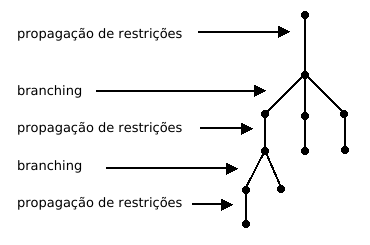
\includegraphics{images/searchtree.png}
  \caption{Exemplo de árvore de busca para um modelo CSP.}
  \label{fig:searchtree}
  \end{figure}

  O procedimento padrão de uma busca top-down é
  o \estr{backtracking}. Ele inicia a busca pelo nó raiz da árvore e
  segue para o primeiro nó descendente. O processo continua até que
  uma folha é encontrada, neste caso, ele retorna para o nó ancestral
  mais próximo que possua outro nó descendente, e então o processo
  recomeça. Se o controle voltou para o nó raiz e todos os
  descendentes foram visitados, o processo termina.

  Um exemplo de \estr{branching} é a técnica conhecida
  como \estr{labelling}, que divide um domínio (finito) de uma
  variável em domínios unitários, correspondendo a uma busca
  sistemática de todos os valores de uma determinada variável. Uma
  forma de propagação de restrições, combinada com o \estr{branching},
  é aplicada ao longo da árvore, removendo valores dos domínios das
  variáveis que não participam de nenhuma solução.}

\end{itemize}
